\documentclass[english,12pt,a4paper]{article}

%%%%%%%%%%%%%%%%%%%%%%%%% packages %%%%%%%%%%%%%%%%%%%%%%%%
\usepackage{amsmath}
\usepackage{amssymb}
\usepackage{mathrsfs}
\usepackage{amsthm}
\usepackage{amsfonts}
\usepackage{graphicx}
\usepackage[T1]{fontenc}
\usepackage[latin9]{inputenc}
\usepackage{textcomp}
\usepackage{listings}
\usepackage[all]{xy}
\usepackage{verbatim}
\usepackage[left=2cm,right=2cm,top=3cm,bottom=2.5cm]{geometry}
\usepackage{float}
%\usepackage{algorithm}
\usepackage[linesnumbered,ruled,vlined]{algorithm2e}

%%%%%%%%%%%%%%%%%%%%% students data %%%%%%%%%%%%%%%%%%%%%%%%
\newcommand{\student}{NONO SAHA Cyrille Merleau}
\newcommand{\course}{Information Geometry}
\newcommand{\assignment}{Assignment II} 
%%%%%%%%%%%%%%%%%%% using theorem style %%%%%%%%%%%%%%%%%%%%
\theoremstyle{definition}
\newtheorem{theorem}{Theorem}
\newtheorem{lemma}[theorem]{Lemma}
\newtheorem{definition}[theorem]{Definition}
\newtheorem{example}[theorem]{Example}
\newtheorem{remark}[theorem]{Remark}
\newtheorem{corollary}[theorem]{Corollary}
\makeatletter
\usepackage{listings}
\usepackage{color}
\lstset{frame=tb,
	language=Python,
	aboveskip=3mm,
	belowskip=3mm,
	showstringspaces=false,
	columns=flexible,
	basicstyle={\small\ttfamily},
	numbers=none,
	numberstyle=\tiny\color{gray},
	keywordstyle=\color{red},
	commentstyle=\color{dkgreen},
	stringstyle=\color{mauve},
	breaklines=true,
	breakatwhitespace=true,
	tabsize=3
}

\definecolor{dkgreen}{rgb}{0,0.6,0}
\definecolor{gray}{rgb}{0.5,0.5,0.5}
\definecolor{mauve}{rgb}{0.58,0,0.82}


%%%%%%%%%%%%%%%%%%%%%%%%%%%%%% LyX specific LaTeX commands.
\newcommand{\lyxmathsym}[1]{\ifmmode\begingroup\def\b@ld{bold}
	\text{\ifx\math@version\b@ld\bfseries\fi#1}\endgroup\else#1\fi}


\makeatother

\usepackage{babel}
\begin{document}
	%%%%%%%%%%%%%%%%%%%%%%% title page %%%%%%%%%%%%%%%%%%%%%%%%%%
	%\thispagestyle{empty}
	\begin{center}
		\textbf{A New EA selection function for an efficient RNA design.\\[0.5cm]
			(Germany, Leipzig)}
		\vspace{1.0cm}
	\end{center}
	
	%%%%%%%%%%%%%%%%%%%%% assignment information %%%%%%%%%%%%%%%%
	\noindent
	\rule{17cm}{0.2cm}\\[0.3cm]
	Name: \ Nono and Matteo \hfill Revision Number: \ I \\[0.1cm]
	Journal: \ \hfill Date: \today\\
	\rule{17cm}{0.05cm}
	
	\section[I.]{Abstract}
	The inverse RNA folding can be understood as a search problem which consists of searching in a space $ S = \big \{A, C, G, U\big \}^l$ one of many RNA sequence (s) that fold (s) into a given target structure of length $l$.
	Solving this problem is a prior stage for RNA design and is still a real challenge in the field of bioengineering. To improve the RNA inverse folding, we investigate an evolutionary framework implementing a new selection function called Min Ensemble Distance (MED) with a mutation operator which allows the user to fit the nucleotides distribution constrains into the mutation parameters. We implement our algorithm into a simple open source python library called \textit{rnaevol} and the result shows that through this approach, the proposed framework can solve complex targets previously unsolvable by any evolution algorithms on the two main datasets used to benchmark our algorithm by surpassing $7/8$ on EteRNA100 dataset and $8/10$ on the non-EteRNA dataset. This result demonstrates that taking into account a selection function different to the objective function can significantly improve the performance of an evolutionary algorithm and helps to understand much better the search space.
	\vspace{1cm}
	
	\textbf{Key words}: RNA design, inverse RNA folding, Evolutionary Algorithm (EA).

	\section{ Introduction and motivation }

An RNA molecule is a string over a four letter alphabet, each letter representing a particular nucleotide base: A for adenine, U for uracil, C for cytosine, and G for guanine and it plays an important role in all cellular processes. For an RNA molecule to perform a biological function it has to fold in a three-dimensional structure which strongly depends on its secondary structure.  Here we consider the inverse folding problem for which the goal is to find one or many RNA sequences that fold into a given target RNA secondary structure. In another terms it can be considered as an optimization problem where a target RNA secondary structure is given and the goal to determine a set of RNA sequences for which the distance between their corresponding secondary structures and the target one is minimized. In the field of modern bioengineering, to be able to design an RNA molecule which performs a specific function, one must first solve the RNA inverse folding problem \cite{goldberg2011nanoparticle}, \cite{hao2014construction}, \cite{win2008higher}.

Many methods  or algorithms addressing this problem have been proposed in the literature and most of them are performing a stochastic search optimization where an initial potential solutions is generated and refined over a finite number of iterations or generation \cite{esmaili2015erd}, \cite{dromi2008reconstruction}, \cite{esmaili2014evolutionary}, \cite{taneda2011modena}, \cite{churkin2017design}. Apart from that there are many other algorithms that are not in the stochastic search basket such as, sentRNA \cite{shi2018sentrna} which is a computational agent for RNA design that uses a set of information and strategies collected from the EteRNA game players to train a neural network model that will be enable to predict a set of sequences folding into a given target structure. It is one of the most recent tools.  antaRNA \cite{kleinkauf2015antarna} utilizes "ant-colony" optimization, in which an initial sequence is generated via a weighted random search, and the goodness of these sequences is then used to refine the weights and improve subsequence over generations. IncaRNAtion generates a GC-weighted partition function for the target structure, and then adaptively samples sequences from it to match a desired GC content. Finally, RNAiFold \cite{garcia2013rnaifold} employs constraint programming that exhaustively searches over all possible sequences compatible with a given target. These approaches have  many advantages and disadvantages depending on the technics implemented. NUPACK \cite{zadeh2011nucleic} for example despite its well defined objective function, still has a difficulty of designing sequences for large targets and most of the EteRNA100 targets recently generated by the online RNA game ETERNA. In contrast, ERD \cite{esmaili2015erd} because of its strong decomposition method which allows it to deal quickly with large targets (On Rfam 1.0 with target's length between $400$-$1400$) but still a big challenge to solve more than $50 \%$ of the ETERNA100 and all other methods are not excluded apart the recent machine learning model sentRNA which was enable to solves $78\%$ of ETERNA100 by adding a refinement on the machine learning model and and without the refinement the deep learning propose by sendRNA can only solve $48\%$ of EteRNA100.

 In this work we are more interested in the class of evolutionary algorithms because through its process we can understand much better the RNA sequences (genotype) - (phenotype) RNA structure mapping which can definitively guide our search method. Many works have been done also in the sense of understanding and characterizing the relation between RNA sequence and structure by letting a population of RNA sequence evolve over generation\cite{ancel2000plasticity} and this can definitively help of designing new evolutionary algorithm to deal much efficiently with the inverse RNA design problem. Amount the methods applying a stochastic search optimization very  few of them belong to the class of evolutionary algorithms \cite{esmaili2015erd}, \cite{esmaili2014evolutionary}, \cite{taneda2011modena} and from our knowledge up to now none of them is able to solve more than $60\%$ of ETERNA100, for that reason we investigate in this work the choice of a selection function for which the performance of an evolutionary algorithm can be significantly improved and we propose a simple evolutionary algorithm implementing most of the objective functions used by previous tools as a selection function and our proposed selection function.  The evolutionary algorihm implements a mutation operation on a population of RNA sequences, the selection is perform by measuring how close to the target structure $\sigma*$ are the structures in the unpseudoknotted structural ensemble $ \Gamma$ of a given sequence $s$ in the population, we call the selection function Min Ensemble Distance (MED). To be able to demonstrate the power of population based algorithm we implemented the Ensemble Defect (ED) selection function (the objective function used by NUPACK ) and discuss some of the results obtained. Finally by benchmarking the evolutionary algorithm on Eterna100 we obtain $71\%$ of success and on $87\%$ on the $63$ target collected from Rfam [...]. This result actually shows how important is the choice of selection function while designing an evolutionary algorithm for  RNA design. 

In the first part of our work, we present the general steps of an evolutionary algorithm for inverse RNA folding problem and we explain the main parts of it which are mutation operation and selection method used. In the second part we discuss the choice of evolutionary algorithm parameters: mutation rates and selection function and in the last part we benchmark the method and compared his performance to other methods in the literature.

	\section{ Evolutionary algorithm approaches to solve Inverse RNA folding}

	\subsection{Method}
The algorithm that we propose in this work consists of three main parts (See Figure \ref{Fig:model}): 

\begin{itemize}
	
	\item  Initialization of the population of RNA sequences 
	\item Selection process
	\item Mutation precess
\begin{figure}[H]
		\centering
		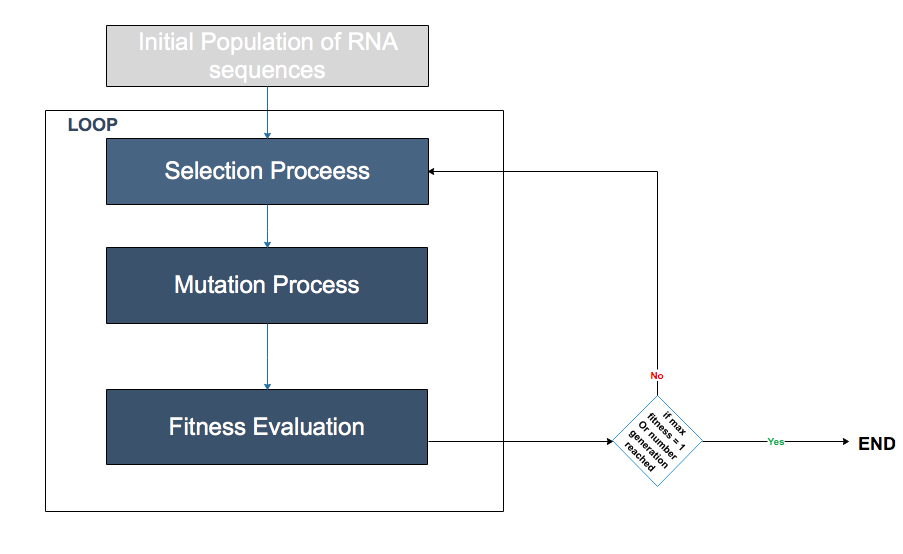
\includegraphics[width=.9\linewidth]{images/model.png}
		\caption{Illustration of an Evolutionary algorithm for RNA design}\label{Fig:model}
		\medskip
		\small.
\end{figure}
	
	
\end{itemize}

\subsubsection{Initialization}
\label{sec:initialization}
For a given population size $N$ and a target structure $\sigma*$ of length $l$, the initial population of our evolutionary algorithm consists of a population of $N$ RNA sequence generated randomly as follows: 

\begin{enumerate}
	\item Select randomly $N$ nucleotides in a set given by $\big\{A, U, G, C \big\}$
	
	\item Identify the base pair position $(i,j)$ in the random sequence previously construct select randomly a base pair in the set of canonic base pairs $\big\{AU, UA, GU, UG, CG, GC \big\}$ and fix the first nucleotide of the selected canonic base pair at the position $i$ and the second at position $j$.
	
	\item  repeat 2. for all base par position in the target structure
	
	\item repeat 1. 2. and 3 $N-$times.
\end{enumerate}

\subsubsection{Selection methods}
	As the natural selection is an important step for all evolutionary processes, selection method (or function) plays also an important role within an evolutionary algorithm. In this work we are presenting a new selection method called Min Ensemble distance (MED). and comparing it to three common selection methods used in the previous woks. In our evolutionary algorithm model four selection functions are considered:  
\begin{itemize}
	\item  Fitness proportion selection: this is the common selection method used by most of the evolutionary algorithm where the objective function is actually use as a selection criteria to know which individual in the current population will be involved in the next generation. Since the main goal of the inverse folding problem is the find sequences that fold into a given target secondary structure $\sigma*$, the simple fitness measurement $f$ of an RNA sequence $\phi$ can be defined as follows:
	
	$$ 
		f(\phi, \sigma*) = \frac{1}{1 + ham(s^{MFE}(\phi) , \sigma*)}
	$$
	Where $ham$ is the hamming distance between the MFE structure $(s^{MFE})$ in the ensemble and the target structure $(\sigma*)$.
	
	$$
		s^{MFE}(\phi) = \arg \min_{s \in \Gamma}\Delta G(\phi, s) 
	$$
	\item Min Ensemble Distance (MED) selection: Here is a new selection function we propose. It is a measure of how close to the target structure $\sigma*$ are the structures in the unpseudoknotted structural ensemble $ \Gamma$ of a given sequence $\phi$ in a population. So what the MED selection does is to preserve in the population most of these  sequences who have in their structural ensemble the target structure or a structure very close to the target one. The  MED selection function measurement is given by:
 	$$
	med(\phi, \sigma*) = \min_{s \in \Gamma(\phi)} ham(s, \sigma*)
	$$
	
	Where $\phi$ is an RNA sequence with base identities $\phi_i \in \big \{ A,C,G, U \big \}$ and $ham(s , \sigma*)$ is the hamming distance between the MFE structure $s$ in in the unpseudoknotted structural ensemble $ \Gamma$ and the target structure $(\sigma*)$
		\item Ensemble defect (ED) selection \cite{zadeh2011nucleic}.
	
	$$ 
	n(\phi, \sigma*) = N - \sum_{1<i,j<N} S_{i,j}(s^{MFE}(\phi))S_{i,j}(\sigma*)
	$$
	Where $S(s)$ is a structure matrix with entries $S_{i,j} \in \big \{ 0, 1\big \}$. If structure $s$ contains pair $\{i \cdot j\}$, then $S_{i,j}(s) = 1$ otherwise $S_{i,j}(s) = 0$. [ref...]

	
%	\item Ensemble diversity (EDV) selection: 
	
%	$$ 
%	d(\phi) = 1 - \sum P_{i,j}^2(\phi)		
%	$$
	
%	Where, 
%	$$ 
%		P_{i,j}(\phi) = \sum_{s\in \Gamma} p(\phi, s)S_{i,j}(s)		
%	$$
%	And 
%	
%	$$
%	p(\phi, s) = \frac{1}{\sum_{s \in \Gamma} \exp(-\Delta G(\phi,s)/k_BT)} \cdot  \exp(-\Delta G(\phi,s)/k_BT)
%	$$
	
	
\end{itemize}

\subsubsection{Mutation operation.}
In this work, we present a correlated mutation under two different mutation rates. We define by $\mu_{bp}$ the probability of each $(i,j)$ base pair position to be mutated and $\mu$ the probability to mutate a non base pair position $i$ in a sequence $(S_i)_{1\leq i \leq N}$.   

Let $ N = \big \{ A, U, C, G \big \} $ be the set of possible nucleotides weighted respectively by a probability:  $$ 
P_N = \big \{ P_A, P_U, P_C, P_G \big\}
$$

 And $C = \big \{  AU, UA, CG, GC, UG, GU\big \}$ be a set of canonic base pairs weighted respectively by a probability:
 
 $$
 P_C = \big \{P_{AU}, P_{UA},P_{CG},P_{GC},P_{UG},P_{UG} \big \} 
 $$
 
 Where, \\
 
  $\sum P_N = 1$, $\sum P_C  = 1$ and $P_{AU} = P_{UA}$, $P_{UG} =P_{GU}$, $P_{CG} = P_{GC}$\\  

The interesting thing with the mutation performed through the evolution algorithm we are proposing in this work is the flexibility of the mutation rate parameters. Our algorithm allows the user to set the designing constraints explicitly through the mutation parameters $P_C$ and $P_N$ which allows to control the nucleotide distribution during the evolutionary process. 
The mutation operation is performed as follows: 

\begin{algorithm}[H]
	\KwData{$(S_i)_{1\leq i \leq N}$, $\mu$, $\mu_{bp}$}
	\KwResult{Mutated sequence }
	$i = 1 $\;
	\While{$i \leq N $}{
		read current\;
		\eIf{ base pair at $(i,j)$}{
			select a random uniform number $r$\;
			\If {$r < \mu_{bp}$}{
				select a canonic base pair $c\in C$ respect to probability $P_C$ \;
				$S[i] = c[1]$\;
				$S[j] = c[2]$\;
			}
		}{
			select a random uniform number $r$\;
			\If {$r < \mu $}{
				select a nucleotide $n_i \in N$ respect to probability $P_N$ \;
				$S[i] = n_i $\;
			}
		}
	$ i = i + 1$\;
	}
	\caption{Mutation algorithm}
\end{algorithm}
%\vspace{1.3cm}

An illustration of the execution of the above algorithm is shown on the Figure \ref{Fig:mut1} bellow.\\
\begin{figure}[H]
		\centering
		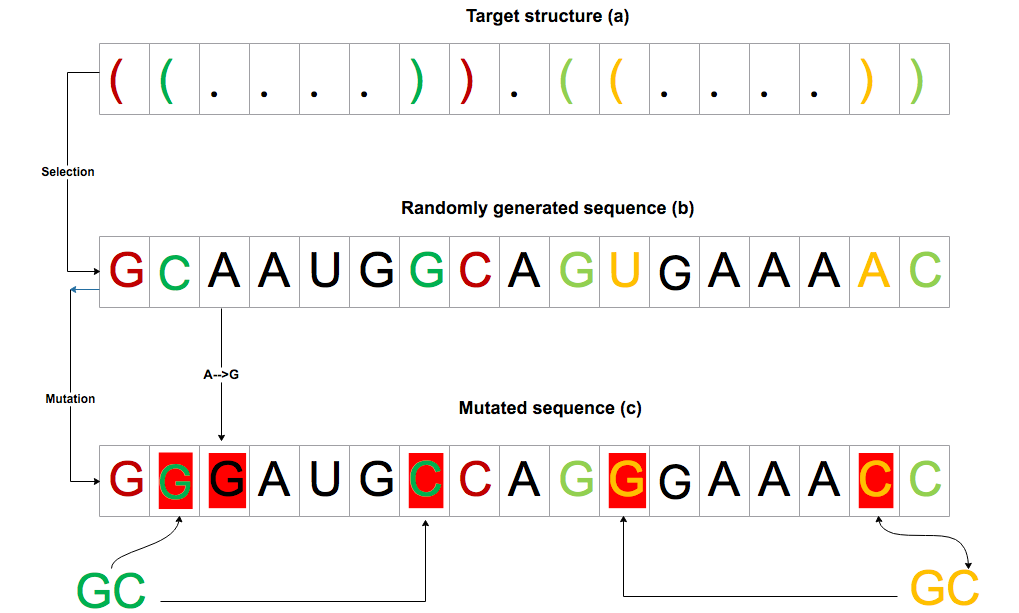
\includegraphics[width=.9\linewidth]{images/mutation_example.png}
		\caption{Illustration of mutation process}\label{Fig:mut1}
		
\end{figure}
\medskip
\small
\textbf{(a)} is a given target structure and \textbf{(b)} is a random generated sequence selected from an N-population of RNA-sequences. \textbf{(c)}  is the mutated sequence where the non-base pair positions (the part in black) are mutated with a probability $\mu = 1/17$, so only one nucleotide has been mutated at the third position $(A-->G)$ . The base pair positions are mutated with a probability $ \mu_{bps}>\mu $ (the coloured part above) four positions have been mutated $(1,6)$ and $(11, 16)$.

To summarize the above steps,  the evolutionary algorithm implementing the selection function we propose is given by: 

\begin{algorithm}[H]
	\KwData{ $N$, $max_{gen}$, $\mu$, $\mu_{bp}$}
	\KwResult{nextpopulation}
	$n = o $\;
	prevpopulation = initipop($N$)\; 
	max\_fitness = max(prevpopulation)\;
	
	\While{$n \leq max_{gen}  \And max\_fitness < 1.0$ } {
		nextpopulation = copy of the $10$ best individuals in prevpopulation\;
		evaluate(prevpopulation)\;
		selected\_ind = select(prevpopulation, size, method)\;
		\For{ind $\in$ selected\_ind}{
		mutated\_ind.add(mutate(ind, $\mu$, $\mu_{bp}$))
		} 
	
		nextpopulation = nextpopulation.add(mutated)\;
		prevpopulation = copy(nextpopulation)\;
		max\_fitness = max(prevpopulation)\;
		$ n = n + 1$\;
	}
	\caption{rnaevol algorithm}
\end{algorithm}

	\section{Results and discussions}
	In this section we would like to address two main parts of our work. First the choice of the evolutionary algorithm parameters, secondly we discuss the importance of the selection function and finally, using two different benchmark data, we compare the results obtained  and the performance of our method to the existent one. In all the experiments carried out in this work, we are using the python library \textit{rnaevol} (implementing our proposed EA framework) which depends on  ViennaRNA Package 2.0 \cite{lorenz2011viennarna} including: RNAfold, RNAsubopt, RNAeval, etc...
	\subsection{ Parameters}

One of the main challenge for an Evolutionary algorithm to perform good result is to find right parameters that fit into the algorithm. The EA proposed in this work  has a set of parameters that need to be tuned. We have: 
\begin{itemize}
	\item The population size $N$ and the number of generation $max_{gen}$: The is always a trade-off between the number of generation and the population size needed by an EA to perform efficiently. In most of the cases less the population size is more we need generation and vice versa. For the matter of resources and to evaluate our algorithm in the worst case the population size we have chosen doest not exceed  $120$ individuals peer generation. in the most case $N = 100$. and $max_{gen} < 500$. 
	\item The mutation parameters $\mu$, $\mu_{bp}$, $P_N$ and $P_C$: For all the experiment we perform in this work $\mu$ is chosen proportionally to the length of the target generally $\frac{1}{\text{lenght of the target}}$  and $\mu_{bp}>>\mu$ for most cases $\mu_{bp} = 0.5$ to allow half of the base pairs positions of a sequence to be mutated. the parameters $P_C$ and $P_N$ are chosen based on the nucleotide distribution in natural RNA in \cite{esmaili2015erd}.
	\item The selection function: For the selection function, the most used is MED function and something switch to the fitness selection function due to the computation time which in our case strongly depends on the length of the target. 
\end{itemize}


\subsection{EA's selection methods analysis}
As mentioned earlier the mains challenge in this work is to choose which of the three selection method is the best for an evolutionary algorithm to solve the inverse RNA folding problem. To compare them we have chosen some target structures from the ETERNA database on which we have performed the following analysis: 

\begin{itemize}
	\item Compare the mean fitnesses over generation over generation.
	\item Counting the number of success over all the experiments performed
	\item For each success, reconstruct the genealogy of the structures and compare their fitness and the mean fitness at  each generation. 
	
\end{itemize}


To be able to compare the three selection methods the first target structure chosen from ENTERNA database is Shortie 6 for two reasons, first because of the short structure length of $35$ which allows us to repeat the experiment many time and secondly because was one of the structure difficult to design and used by Jeff and al in \cite{anderson2016principles} to compare RNA-design tools such as NUPACK, INFIO-RNA, RNA-Inverse, RNA-SSD, etc... 

The Table bellow summarizes the result. 

\begin{table}[H]
	\caption{Comparison of selection methods on Short 6} \label{table1}
	
	\hspace{1cm}
	\begin{tabular}[H]{|c|c|c|c|}%c|}
		\hline
		\textbf{Selection methods}& Ens Def. & Min Ens Dist. & Fitness\\%& Ens diversity\\
		\hline
		\textbf{Average number of generations}&$229.84$&$280.59$&$500$\\%&$500$ \\
		\hline
		\textbf{Median number of generations}&$192.$&$236$&$500$\\%&$500$ \\
		\hline
		\textbf{Number od success}&$90$&$67$&$0$\\%&$0$\\
		\hline
		
	\end{tabular}
\end{table}
\medskip
\small 
The result above is obtained by repeating $100$ times, for a maximum of $500$ generations, the mutation probabilities $\mu = \frac{1}{35}$ and $\mu_{bp} = 0.5$ without elitism and using an initial population generated using the steps above section  \ref{sec:initialization}.  The Table \ref{table1} shows that the ED selection method solves with a success rate of $90\%$  and the MED follows with a success rate of $67\%$. 

The surprising observation that we can make here is that in the paper of Jeff et al. \cite{anderson2016principles}  where the authors compared the existing tools by benchmarking them on Eterna100 the tool NUPACK which solves the inverse folding by minimizing the ensemble defect did not solve this structure, so which means that through an evolutionary algorithm where the selection function minimizes the ensemble defect can perform better. 

The Figure \ref{Fig:MED1} \textbf{(a)} bellow show that for one of the success run the ensemble defect of the sequence found is actually less than the one obtained by running the same structure on the last version of NUPACK web server. The sequence found by NUPACK web server is given by: $$GGAAUACCAGAGAGAUCAGCGUUUGCACCACCUGG$$ and using the RNAfold tool from ViennaRNA package the sequence folds into the following structure:
$$......((((.(......((....))....))))) ( -3.10)$$
And the corresponding  ensemble defect is $15.58$ which is higher that the one obtained by our method which is under $8.0$. as we can observe on Figure \ref{Fig:MED1} \textbf{(a)}.
\begin{figure}[H] 
	\vspace{-0.3cm}
	\hspace{-1.2cm}
	\begin{minipage}{0.60\textwidth}
		\centering
		\textbf{(a)}\label{Fig:small1}
		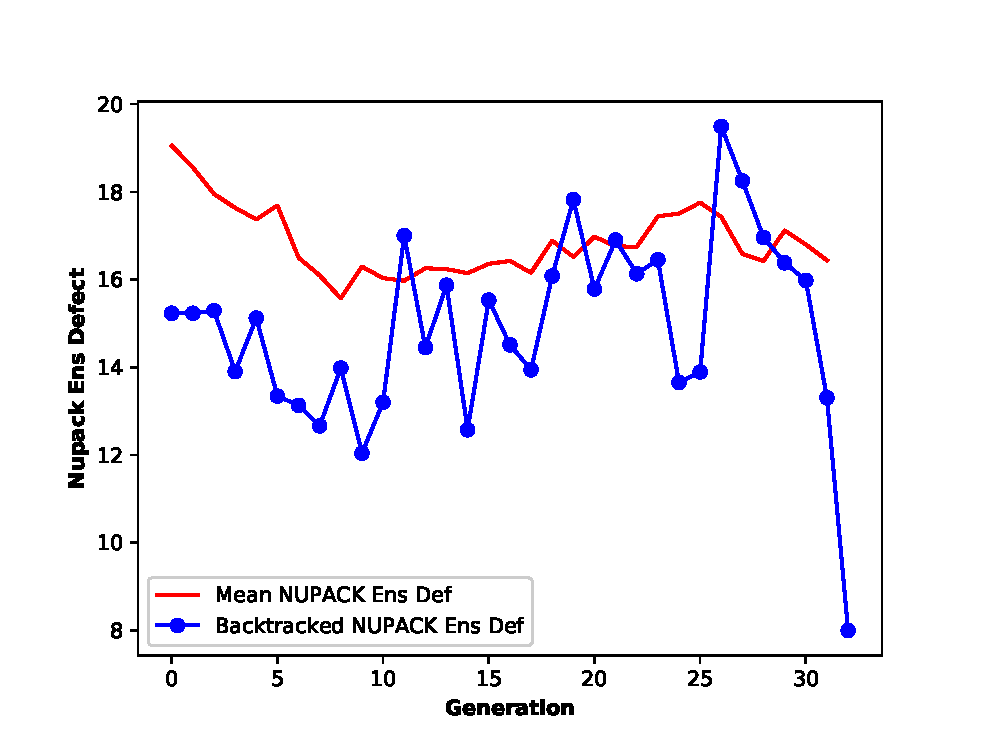
\includegraphics[width=.9\linewidth]{images/stat1-65}
	\end{minipage}\hfill
	\begin{minipage}{0.6\textwidth}
		\centering
		
		\textbf{(b)}\label{Fig:small2}
		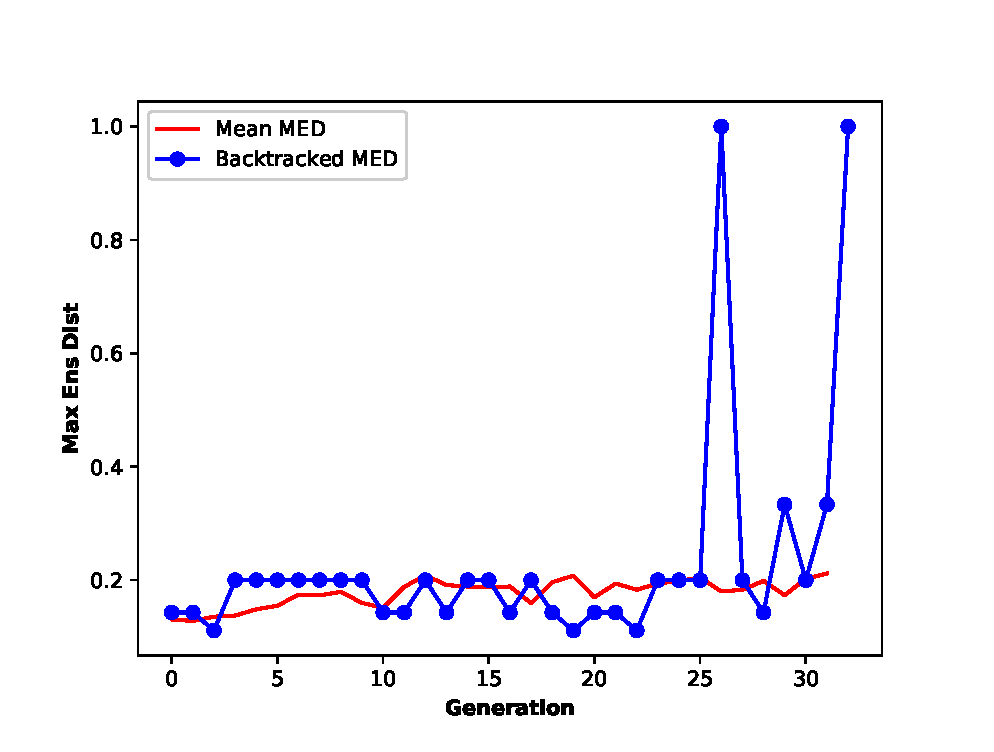
\includegraphics[width=.9\linewidth]{images/stat4-65}
	\end{minipage}
	
	\hspace{-1.2cm}
	\begin{minipage}{0.60\textwidth}
		\centering
		\textbf{(c)}\label{Fig:small3}
		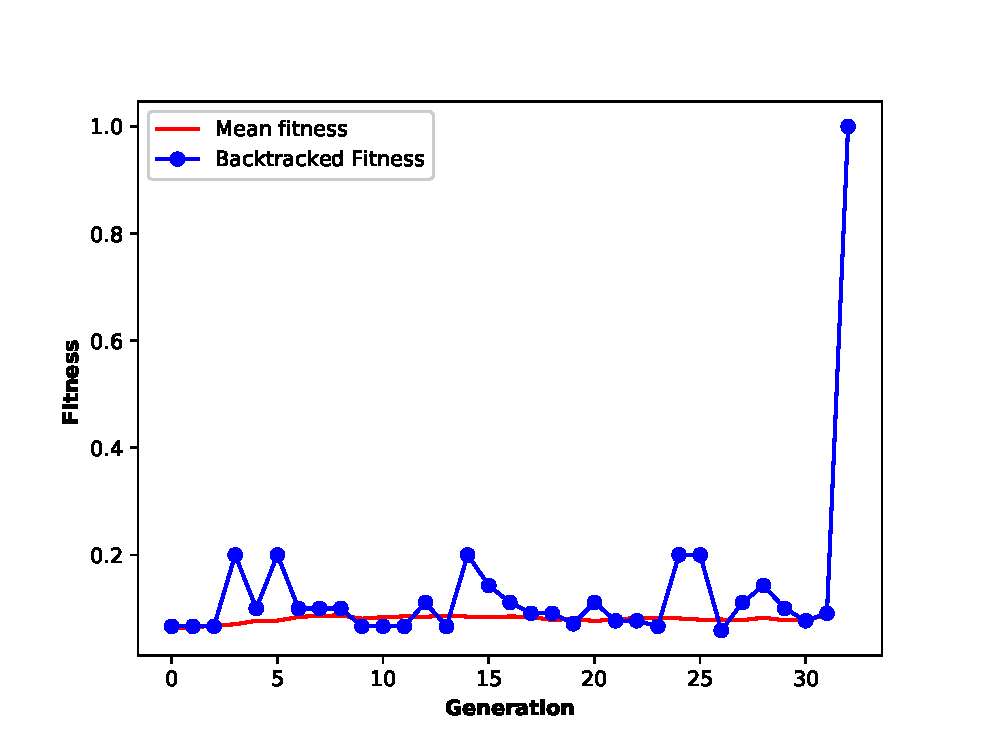
\includegraphics[width=.9\linewidth]{images/stat3-65}
	\end{minipage}\hfill
	\begin{minipage}{0.6\textwidth}
		\centering
		
		\textbf{(d)}\label{Fig:small4}
		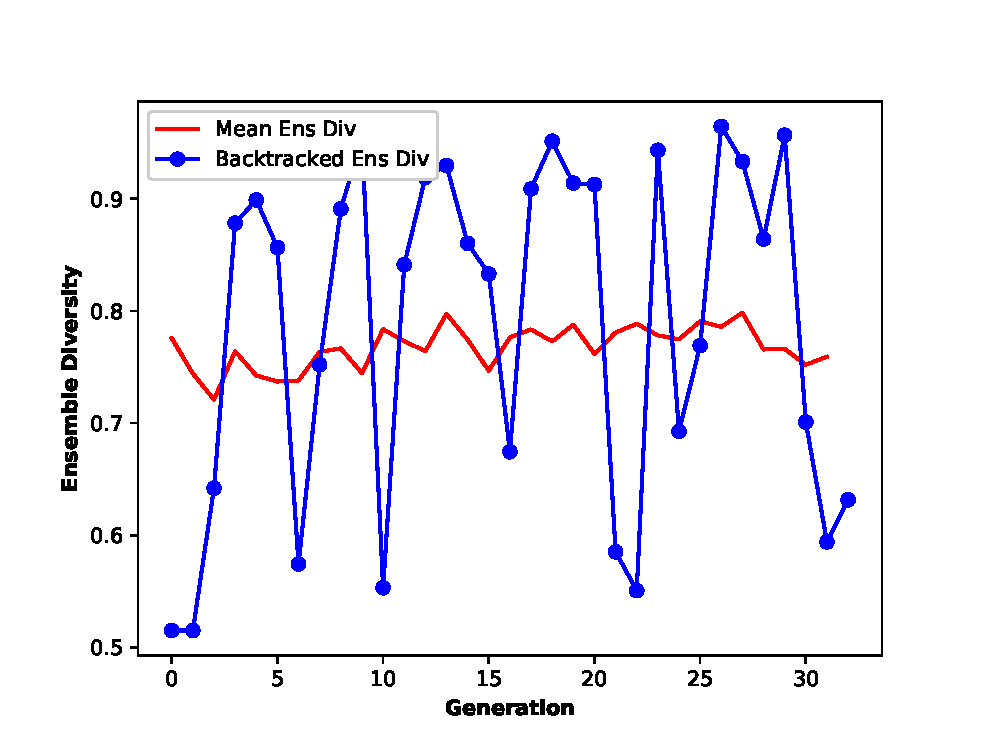
\includegraphics[width=.9\linewidth]{images/stat2-65}
	\end{minipage}
	
	\caption{Shortie 6 structure analysis.}\label{Fig:MED1}
	
\end{figure}
\medskip
\small
\textbf{(a)} is showing the mean ensemble defect of a population od $100$  sequences over generation compared to the ensemble defect of all sequence in the genealogy of the found structure,   \textbf{(b)} the min ensemble distance, \textbf{(c)}  the  fitness and the last plot \textbf{(d)} shows the means ensemble diversity compared to the ensemble diversity of backtracked sequences. As we can observe for this run that the ensemble defect and the min ensemble distance selection methods seems to be promising. Firstly because on \textbf{(a)} and  \textbf{(b)} most of the backtracked sequences ensemble defects computed are bellow the mean ensemble and the same for the min ensemble distance they are above. Further more, if we look at the last sequences before we hit the target structure they are bellow the mean for the ED and above for the MED. In contrast on  \textbf{(d)} is not the same case for the ensemble diversity which was expected to be above the mean too. 

On Figure \ref{Fig:SUM} bellow we have a plot summarizing the $90$ success runs for ED selection and on Figure \ref{Fig:SUM2} the $67$ success runs for MED selection method.  

\begin{figure}[H] 
	\vspace{-0.1cm}
	\hspace{-1.2cm}
	\begin{minipage}{0.60\textwidth}
		\centering
		\textbf{(a)}\label{Fig:small1}
		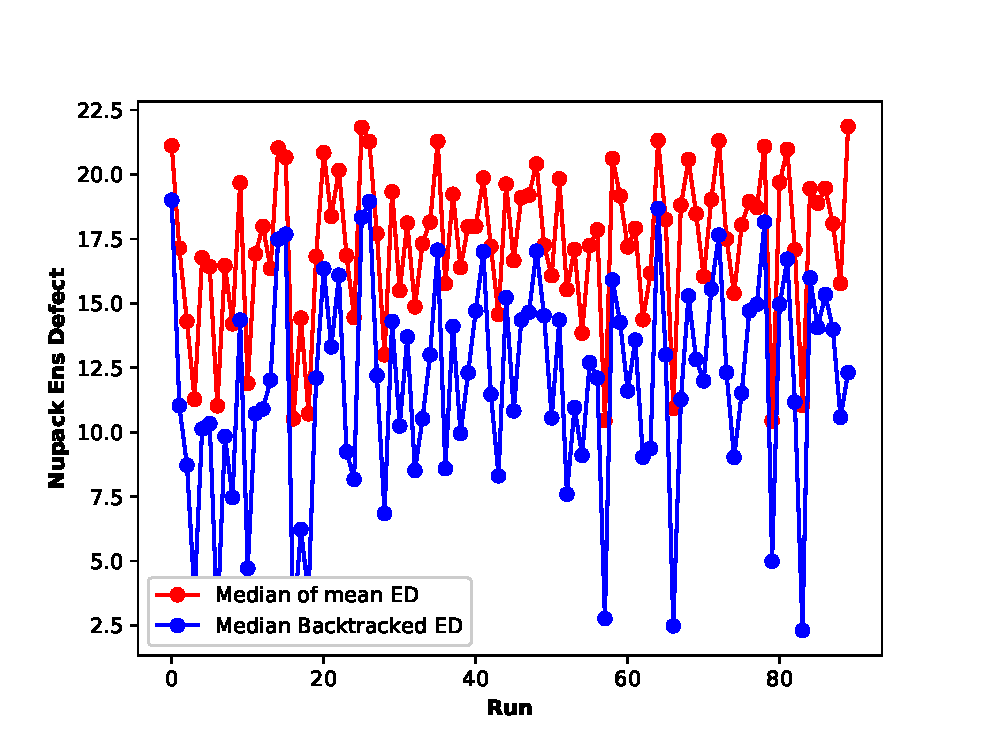
\includegraphics[width=.9\linewidth]{images/41-2/1/stat1-48}
	\end{minipage}\hfill
	\begin{minipage}{0.6\textwidth}
		\centering
		
		\textbf{(b)}\label{Fig:small2}
		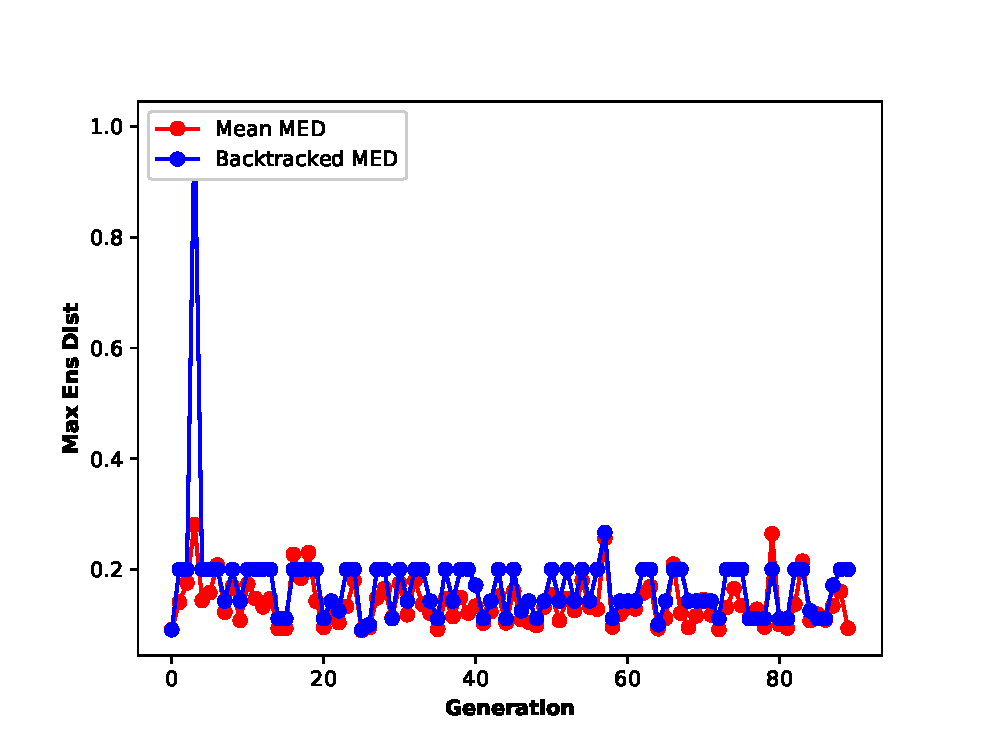
\includegraphics[width=.9\linewidth]{images/41-2/1/stat4-48}
	\end{minipage}
	
	\caption{Shortie 6 structure analysis for the $90$ success run of  ED's selection method.}\label{Fig:SUM}
	\medskip
	\small
	\textbf{(a)} is showing for each success run in blue the median of the distribution of backtracked sequences ensemble defect and in red the median of the distribution of mean ensemble defect in a population of $100$  sequences over generation and on  \textbf{(b)} the same observation for the min ensemble distance. 
	
	
\end{figure}
\begin{figure}[H] 
	\vspace{-0.5cm}
	\hspace{-1.2cm}
	\begin{minipage}{0.60\textwidth}
		\centering
		\textbf{(a)}\label{Fig:small1}
		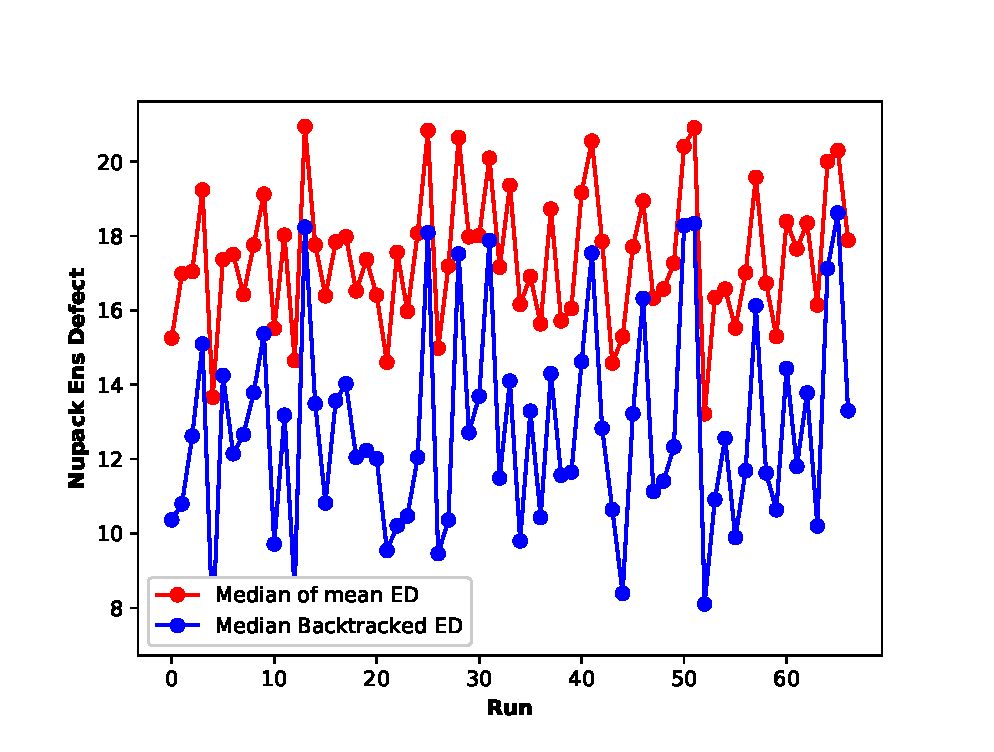
\includegraphics[width=.9\linewidth]{images/41-2/2/stat1-48}
	\end{minipage}\hfill
	\begin{minipage}{0.6\textwidth}
		\centering
		
		\textbf{(b)}\label{Fig:small2}
		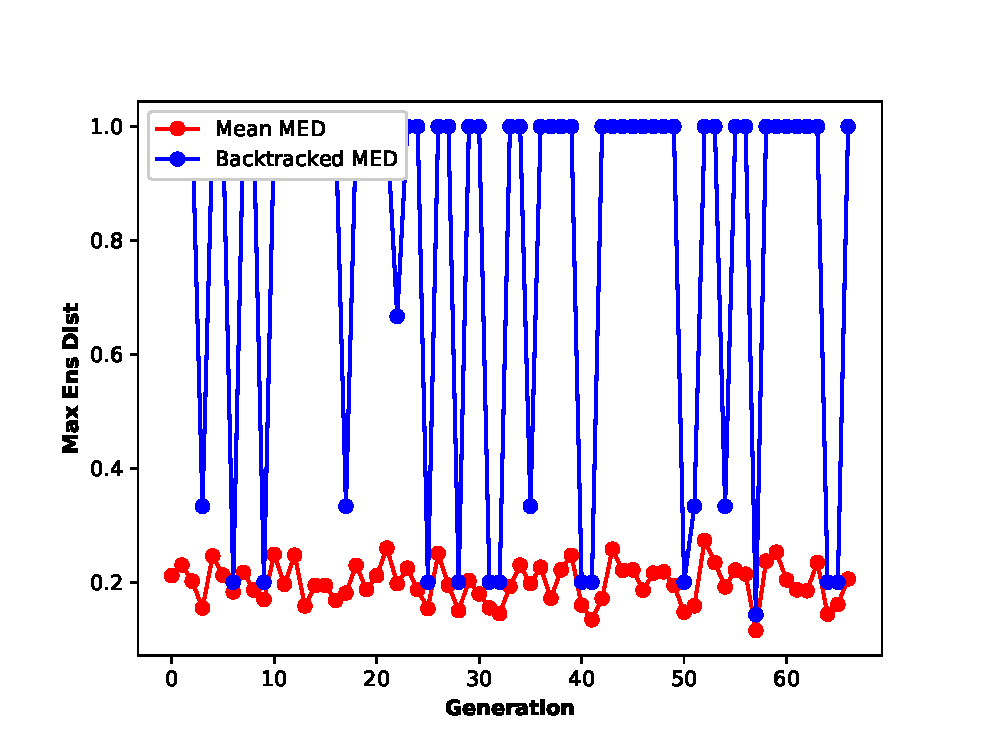
\includegraphics[width=.9\linewidth]{images/41-2/2/stat4-48}
	\end{minipage}
	
	\caption{Shortie 6 structure analysis for the $67$ success run of  MED's selection}\label{Fig:SUM2}
	\medskip
	\small
	\textbf{(a)} is showing for each success run in blue the median of the distribution of backtracked sequences ensemble defect and in red the median of the distribution of mean ensemble defect in a population of $100$  sequences over generation and on  \textbf{(b)} the same observation for the min ensemble distance 
	

\end{figure}

As explained earlier for one MED success run, we can make the same observation for all the success runs of each method on Figure \ref{Fig:SUM} and Figure \ref{Fig:SUM2} which show in both cases that for the majority of success runs the median of ensemble defect and the min ensemble distance of backtracked sequences are respectively bellow the median of the mean distribution of ED in the population and above  the median of the mean ensemble. 

We repeated the same experiment above on a different target structure chosen from ENTERNA database called \textit{Small and Easy 6 }for the same reasons as the first one.

The Table bellow summarizes the result. 

\begin{table}[H]
	\caption{Comparison of selection methods on Small and Easy 6} \label{table2}
	\hspace{1cm}
	\begin{tabular}[H]{|c|c|c|c|}%c|}
		\hline
		\textbf{Selection methods}& Ens Def. & Min Ens Dist. & Fitness\\%& Ens diversity\\
		\hline
		\textbf{Average number of generations}&$486.48$&$456.97$&$450.04$\\%&$500$ \\
		\hline
		\textbf{Median number of generations}&$500$&$500$&$500$\\ %&$500$ \\
		\hline
		\textbf{Number od success}&$6$&$17$&$14$\\%&$0$\\
		\hline
		
	\end{tabular}
\end{table}
\medskip
\small 
The result above is obtained by repeating $100$ times, for a maximum of $500$ generations, the mutation probabilities $\mu = \frac{1}{30}$ and $\mu_{bp} = 0.5$ without elitism and using an initial population generated using the steps above section  \ref{sec:initialization}.  As we can notice in Table \ref{table2} the success rate for this second target structure is much lower than the preview one. The ED's selection method is the least one with $6\%$ of success. But it is also important to notice that after $100$ runs using  NUPACK tool we did not get success and the best sequence designed by NUPACK is: 
$$AAUGCGUCAUGCUAUCCAUCUGCGGGAAUU$$ and using the RNAfold tool from ViennaRNA package the sequence folds into the following structure:
$$......((.(((.........))).))... ( -2.00)$$
And the corresponding  ensemble defect is $9.75$ which is higher that the one obtained by our method which is bellow $5.0$ as we can see on the Figure \ref{Fig:small_and_easy6} \textbf{(a)}. 

Performing the same analysis as previously, we can notice from Figure \ref{Fig:small_and_easy6} the same behaviour for one of the success run. Despite of low success rate of ED's method  the ensemble defect selection method seems to be more promising that MED because the ensemble defect of all the backtracked sequences is significantly bellow the mean ensemble defect of the population which shows that maintaining a population of sequences with  low ensemble defect will definitely help to hit the the sequence folding into the target structure. It also important to say that it is almost the same case for the MED selection method.

The plots summarizing the $6$ success runs of ED's method and the $17$ are also shown bellow on Figure \ref{Fig:SUM1-SE6} and Figure \ref{Fig:SUM2-SE6}.
\begin{figure}[H]

	\hspace{-1.2cm}
	\begin{minipage}{0.60\textwidth}
		\centering
		\textbf{(a)}\label{Fig:Data1}
		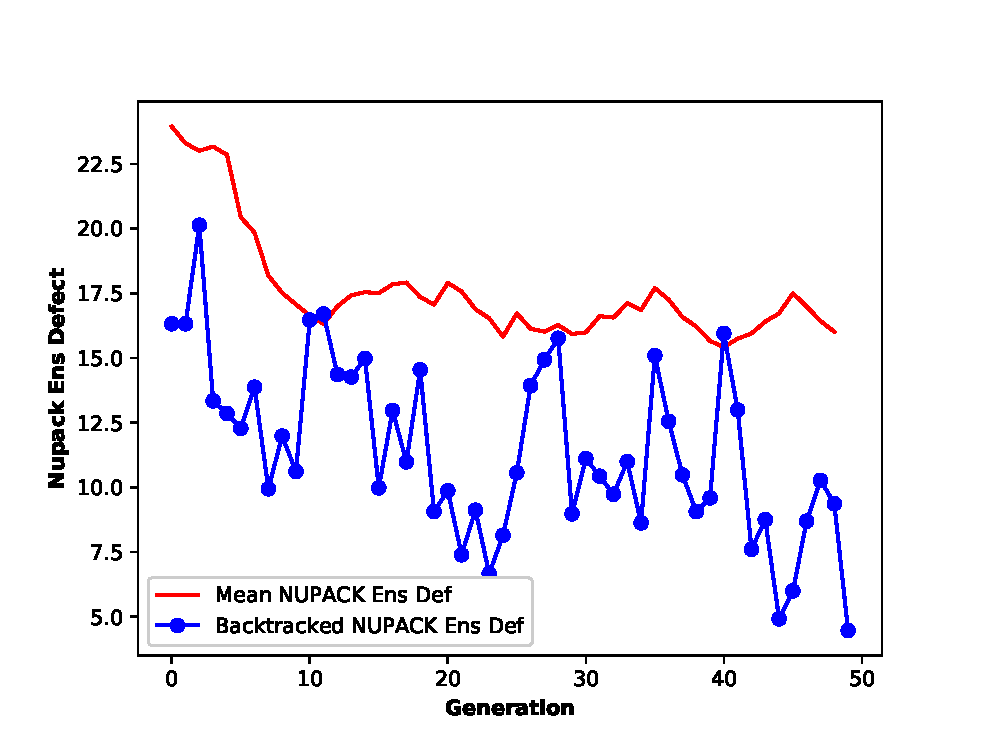
\includegraphics[width=.9\linewidth]{images/stat1-48}
	\end{minipage}\hfill
	\begin{minipage}{0.6\textwidth}
		\centering
		
		\textbf{(b)}\label{Fig:Data2}
		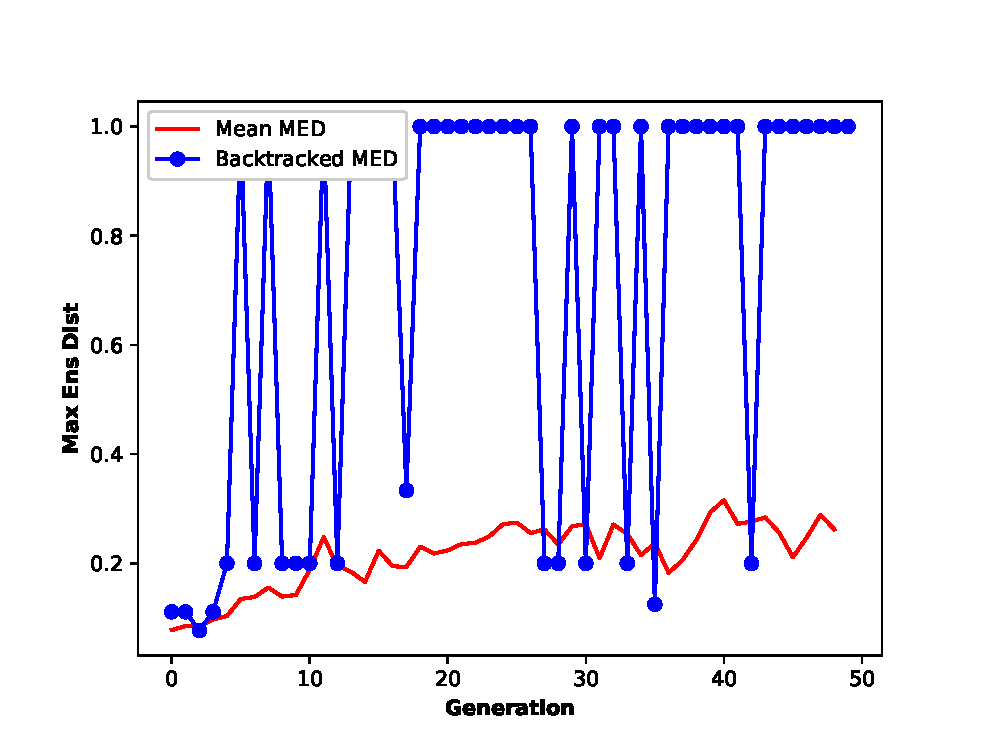
\includegraphics[width=.9\linewidth]{images/stat4-48}
	\end{minipage}

	\caption{Small and Easy 6 structure analysis.}\label{Fig:small_and_easy6}
	
\end{figure}

\begin{figure}[H] 
	\vspace{-0.5cm}
	\hspace{-1.2cm}
	\begin{minipage}{0.60\textwidth}
		\centering
		\textbf{(a)}\label{Fig:small1}
		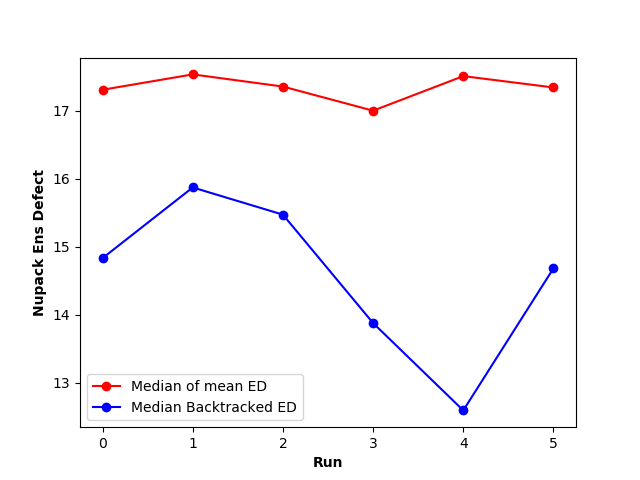
\includegraphics[width=.9\linewidth]{images/data-17-ED/stat1-48}
	\end{minipage}\hfill
	\begin{minipage}{0.6\textwidth}
		\centering
		
		\textbf{(b)}\label{Fig:small2}
		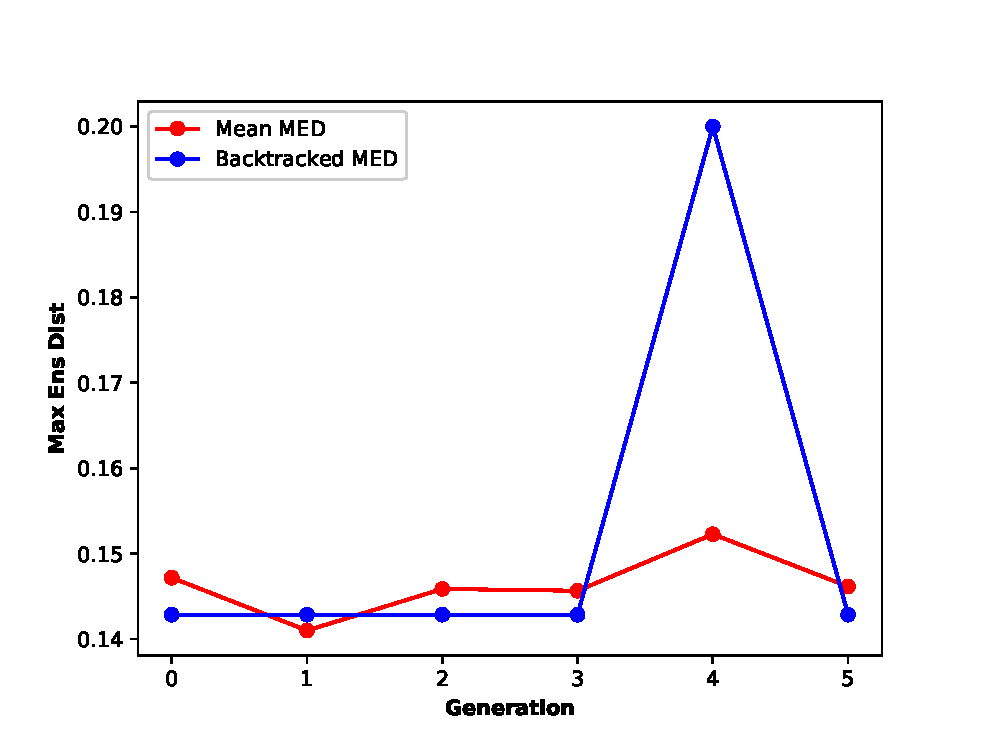
\includegraphics[width=.9\linewidth]{images/data-17-ED/stat4-48}
	\end{minipage}
	
	\caption{Small and Easy 6 structure analysis for the $9$ success run of  ED's selection method.}\label{Fig:SUM2-SE6}
	\medskip
	\small
	\textbf{(a)} is showing for each success run in blue the median of the distribution of backtracked sequences ensemble defect and in red the median of the distribution of mean ensemble defect in a population of $100$  sequences over generation and on  \textbf{(b)} the same observation for the min ensemble distance. On \textbf{(b)} we can notice that in most case the median of the backtracked  sequences is not greater than the median of the mean distribution which makes sense because the selection pressure was on ensemble defect.
	
	
\end{figure}
\begin{figure}[H] 
	\vspace{-0.5cm}
	\hspace{-1.2cm}
	\begin{minipage}{0.60\textwidth}
		\centering
		\textbf{(a)}\label{Fig:small1}
		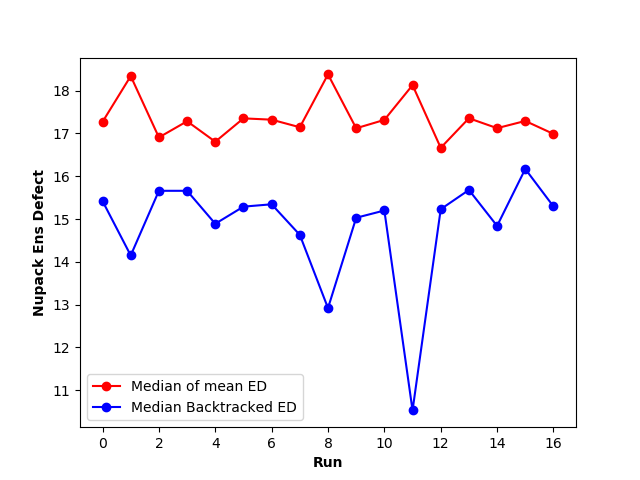
\includegraphics[width=.9\linewidth]{images/data-17-MED/stat1-48}
	\end{minipage}\hfill
	\begin{minipage}{0.6\textwidth}
		\centering
		
		\textbf{(b)}\label{Fig:small2}
		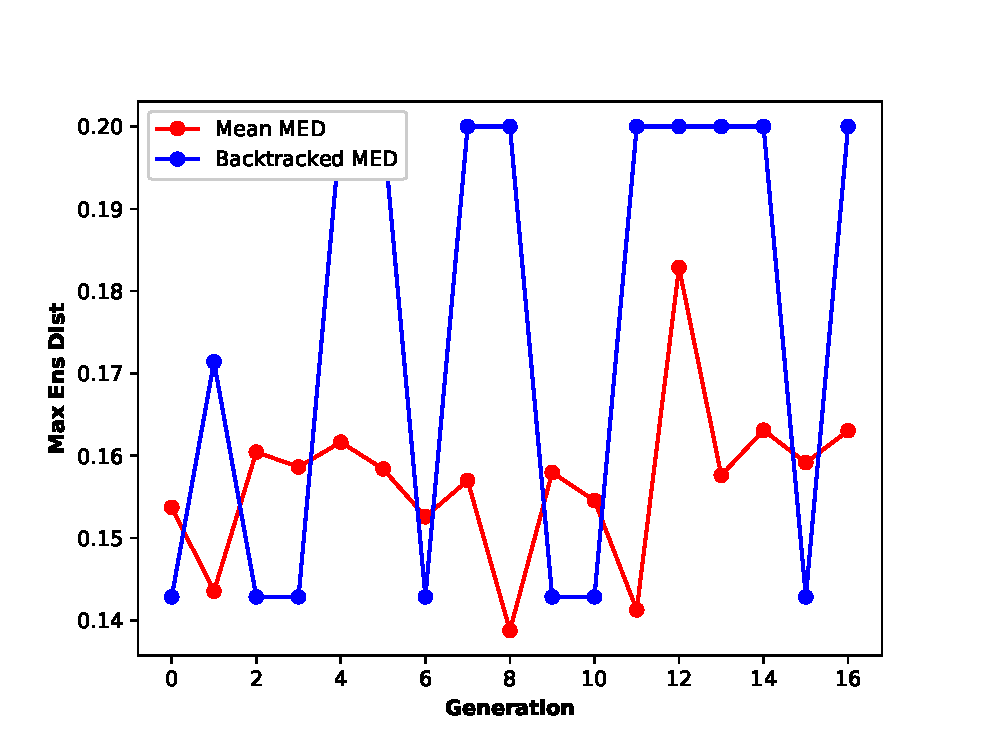
\includegraphics[width=.9\linewidth]{images/data-17-MED/stat4-48}
	\end{minipage}
	
	\caption{Small and Easy 6 structure analysis for the $17$ success run of  MED's selection}\label{Fig:SUM1-SE6}
	\medskip
	\small
	\textbf{(a)} is showing for each success run in blue the median of the distribution of backtracked sequences ensemble defect and in red the median of the distribution of mean ensemble defect in a population of $100$  sequences over generation and on  \textbf{(b)} the same observation for the min ensemble distance. In contrast of the previous one, on \textbf{(a)} we can notice that in most case the median of ED backtracked  sequences is not less than the median of the mean ED distribution which means that some how selecting on MED is also minimizing the ED.
	
	
\end{figure}
\newpage
\subsection{Benchmark}
As we can notice from the previous preformed  experiments , we can not really decide which of the selection methods perform better or is well suited for an EA to deal on inverse folding because in a Shortie 6 the ensemble defect perform better and in a Small and short 6 the MED performs better. So it is important to benchmark them using the entire dataset and compare their result to existing methods. 

\subsubsection{Data description} 
To evaluate and compare the performance of the EA proposed in this work to other existing methods in the literature we have have chosen to use the two main datasets used by the recent tool deep learning tool SentRNA \cite{shi2018sentrna}:

\begin{itemize}
	\item The Eterna100 which contains a set of 100 target structures extracted from Eterna Pulzze game players and classifier by their degree of difficulty. 
	
	\item A set of 63 non-Eterna experimentally synthesized targets that Garcia-Martin et al. recently used to benchmark a set of 10 inverse folding algorithms which for  our knowledge, this is the most recent and comprehensive benchmark of current state-of-the-art methods as also mentioned in \cite{shi2018sentrna}. The dataset is collected from $3$ sources:  the first dataset called \textbf{dataset A} which contains $29$ targets \cite{esmaili2015erd} \cite{taneda2011modena} and the second called \textbf{dataset B} is a collection of $24$ targets used in \cite{esmaili2015erd}  and added to that the $10$ used in \cite{shi2018sentrna}.
	
\end{itemize}
\subsubsection{First observations}
In this first observation, we compare  our EA's performance on the Eterna100 benchmark dataset.  The result in Table 3 bellow is obtained by running in parallel for each target structure  $\sigma*$ in the EteRNA100 $4$ instances of our EA, for a maximum of $200$ generations under a mutation rate of $\mu = \frac{1}{lenght(\sigma*)}$ and $\mu_{bp} = 0.5$ with elitism and using an initial population of $100$ RNA sequences generated using the above steps in section  \ref{sec:initialization}.  In the following table, "\textit{rnaevol + GC pairing}"  corresponds to the mutation parameter $P_N = \big[P_A=0.3,P_U= 0., P_C=0.,P_G=0.7\big]$ and 
$ P_C = \big[ P_{AU}=P_{UA}=0,P_{CG}=P_{GC}=0.5,P_{UG}=P_{UG}=0 \big] $, for the case "\textit{rnaevol + All pairing}"  all the nucleotides have the same chance of being selected and the base pairs as well.

As we can notice in the Table \ref{Table:EternaTest}  the  evolution algorithm we propose, can solve $71\%$ using $MED$'s selection method and $64 \%$  using $ED$'s selection method which is sufficient to surpass $6/7$ methods benchmarked by ER et al. in \cite{shi2018sentrna}. The performances of an EA using the MED's selection method  with all pairing and the one using only GC pairing are almost the same  Using an ED's selection  + GC, we can actually solve $23$ targets more than NUPACK which is also minimizing the ensemble defect and that shows the importance of population based algorithm.  Our proposed EA with a new selection function MEA can solve $17$ target more than the previous GA-based algorithms MODENA \cite{taneda2011modena} \cite{esmaili2014evolutionary}.

\begin{center}
\begin{table}[H]
	\caption{Summary of performance of rnaevol vs the 7 other algorithms benchmarked on the Eterna100 by Anderson-Lee et al. }\label{Table:EternaTest}
	
	\vspace{0.5cm}
	\hspace{1.5cm}
	\begin{tabular}[H]{|c|c|}
		\hline
		\text{Methods}& Number of puzzles solved\\
		\hline
		\textbf{rnaevol with MED selection + GC pairing}&$\textbf{71/100}$\\
		\hline
		\text{rnaevol with MED selection + All pairing}&$\text{60/100}$\\
		\hline
		\textbf{rnaevol with ED selection + GC pairing}&$\textbf{67/100}$\\
		\hline
		\text{rnaevol with ED selection + All pairing}&$\text{50/100}$\\
		\hline
		\text{SentRNA, NN only}&$47/100$\\
		\hline
		\text{SentRNA, NN + full moveset }&$78/100$\\
		\hline
		\text{SentRNA, NN + GC pairing }&$74/100$\\
		\hline
		\text{SentRNA, NN + All pairing }&$72/100$\\
		\hline
		\text{RNAinverse}&$28/100$\\
		\hline
		\text{RNA-SSD }&$27/100$\\
		\hline
		\text{DSS-Opt }&$47/100$\\
		\hline
		\text{NUPACK}&$48/100$\\
		\hline
		\text{INFO-RNA }&$50/100$\\
		\hline
		\text{MODENA }&$54/100$\\
		\hline
		
	\end{tabular}
\end{table}
\end{center}

\subsubsection{Second  observations}
For this second experiment carried out we use the second dataset of $63$ targets structures which is a combination of dataset A and dataset B. The statical result compared to others tools is presented in Table \ref{Tab4:non-eterna}. 

We use the same parameters like in the first experiment apart from the number of generation which is reduce to $100$ and the mutation parameters $P_C$ and $P_N$. $P_C$ and $P_N$ were chosen to be close to the nucleotide distribution of the RNA sequence in the nature \cite{esmaili2015erd}. The result shows that our method surpasses $8/10$ other methods. ERD is solving $2$ targets more than our method because as we stated earlier one of the main advantage of ERD is its strong decomposition capacity which allows it to solve the entire dataset B. For the reason that the targets are very long in the dataset B we used the fitness selection method which allows us to speed up and with the advantage that our evolutionary algorithm also allows us to fit the nucleotide distribution parameters taken from natural RNA directly in the mutation parameters, we are able to solve $21/24$ targets from this \textbf{dataset B}. For the \textbf{dataset A} we use the MED selection method and we solve $24/29$ target which means $2$ more than the previous tools and for the $10$ last targets we solve $7/10$. Adding all this solved target together we obtain a result of $52/63$ presented in Table \ref{Tab4:non-eterna}

\begin{center}
	\begin{table}[H]
		\caption{Summary of performance of rnaevol vs the $10$ other algorithms benchmarked on the non-Eterna100 by Anderson-Lee et al. } \label{Tab4:non-eterna}
		\vspace{0.5cm}
		\hspace{2.5cm}
		\begin{tabular}[H]{|c|c|}
			\hline
			\textbf{Methods}& Number of puzzles solved\\
			\hline
			\textbf{RNAEVOL}&$\textbf{52/63}$\\
			\hline
			\text{SentRNA, NN only}&$46/63$\\
			\hline
			\text{SentRNA, NN + full moveset }&$57/63$\\
			\hline
			\text{SentRNA, NN + GC pairing }&$53/63$\\
			\hline
			\text{SentRNA, NN + All pairing }&$53/63$\\
			\hline
			\text{RNAfbinv}&$0/63$\\
			\hline
			\text{IncaRNAtion}&$28/63$\\
			\hline
			\text{Frnakenstein }&$27/63$\\
			\hline
			\text{RNAinverse}&$20/63$\\
			\hline
			\text{RNA-SSD }&$47/63$\\
			\hline
			\text{NUPACK}&$29/63$\\
			\hline
			\text{INFO-RNA }&$45/63$\\
			\hline
			\text{MODENA }&$32/63$\\
			\hline
			\text{ERD }&$54/63$\\
			\hline
			
		\end{tabular}
	\end{table}
\end{center}


\subsubsection{Accuracy and speed comparisons on the dataset A}

After benchmarking our algorithm on existent datasets and compare the result obtained to previous tools, we also found important to address the accuracy and the speed comparisons of our methods. Here we present time ans accuracy comparison on the \textbf{dataset A}. The formula used to compute $E_t(s)$ is the same used in \cite{esmaili2015erd} and it is given by: 

$$
	E_t(s) = \frac{ \text{Total Excution Time}}{Sc}
$$
And it is important to say that we did not run the experiment on all other tools we took the result performed in \cite{esmaili2015erd}. 

In Table, the best results are indicated in bold, as we can see the $2$ targets: \textbf{RF00028} and \textbf{RF00028} that our algorithm was able to solve more than INFO-RNA and MODENA and the $2$ targets: \textbf{RF00030} and \textbf{RF00018} more than ERD. This allows our algorithm to obtain a best accuracy over all other existing algorithm found in the literature. But we can also notice that even though for a very few cases we have gotten better speed, the computational time is much more expensive than ERD and INFO-RNA and this can be understood by the fact that when we use a selection function different to the fitness function we evaluate every individual tweest at each generation and for a long target we have an exponential growth of the unpseudoknotted structural ensemble $ \Gamma$ of a given sequence in the population and an energy range which consequently increase exponentially the computation time of our algorithm. To avoid an infinite time computation for long targets we set the the maximum energy of each structure in the ensemble $\Gamma$ up to $3$  $Kcal.mol^-1$.

\begin{center}
	\begin{table}[H]
		\caption{Summary of performance of \textit{rnaevol} vs the 4 other algorithms benchmarked on the \textbf{dataset B} by A.Esamaili-Taheri et al} \label{Tab5:speedandaccuracy}
	
		\vspace{0.5cm}
		\hspace{-1.6cm}
		\begin{tabular}[H]{p{1.2cm}ccccccccccc|}
			\hline
			\textbf{ID}&Length(nt)&  \multicolumn{2}{c}{rnaevol} &\multicolumn{2}{c}{ERD} &\multicolumn{2}{c} {INFO-RNA}& \multicolumn{2}{c} {MODENA}&\multicolumn{2}{c}{NUPACK}\\
			
			&&$E_t(s)$&$SC$&$E_t(s)$&$SC$&$E_t(s)$&$SC$&$E_t(s)$&$SC$&$E_t(s)$&$SC$\\
			\hline
			RF00008&54&0.115&50&0.16&50&0.011&50&41.905&49&7.005&50\\
			\hline
			RF00029&73&0.371&50&0.373&50&0.033&50&71.502&38&41.415&41\\
			\hline
			RF00005 &74&0.227&50&0.045&50&0.032&50&36.046&47&24.85 &50\\
			\hline
			RF00027 &79&0.2088&50&0.1&50&0.119&50&61.825 &40&20.732& 50\\
			\hline
			RF00019 &83&0.336&50&0.136&50&0.091&50&50.813&35&9.211&50\\
			\hline
			RF00014 &87&0.2914&50&0.103&50&0.034&50&63.707&35&6.389&50\\
			\hline
			RF00006 &89&0.4&50&0.23&50&0.255&50&37.926&41&51.291&50\\
			\hline
			RF00026 &102&0.36&50&0.038&50&11.294&50&57.124&44&209.624&50\\
			\hline
			RF00001 &117&1,51&50&2.389&49&0.255&50&53.41&46&25423.278&1\\
			\hline
			RF00021 &118&0.556&50&0.3&50&0.164&50&59.139&46&18.411&50\\
			\hline
			RF00020&119&$\infty$&0&$\infty$&0&$\infty$&0&$\infty$&0&$\infty$&0\\
			\hline
			RF00016&129&$\infty$&0&$\infty$&0&$\infty$&0&$\infty$&0&4028.944&7\\
			\hline
			RF00015 &140&2.46&50&2.218 &49&2.885&50&77.096&42&$\infty$&0\\
			\hline
			RF00022 &148&\textbf{2.01}&\textbf{50}&2.846 &50&6.384&50&77.024&44&1870.129&14\\
			\hline
			RF00002 &151&\textbf{3.76}&\textbf{50}&7.831&49&11.294&50&64.602&39&$\infty$&0\\
			\hline
			RF00007 &154&2.64&50&1.429 &50&0.975&50&85.534&43&531.148&32\\
			\hline
			RF00003&161&34,62&34&23.325&43&379.851&14&$\infty$&0&$\infty$&0\\
			\hline
			RF00013 &185&5.92&50&3.014&50&8.601&50&104.908&46&18.1&50\\
			\hline
			RF00004 &193&6,24&50&3.177&50&5.883&50&84.767&41&814.047&14\\
			\hline
			RF00025 &210&11,34&50&7.584&50&7.361&50&106.894&48&$\infty$&0\\
			\hline
			RF00012 &215&13.8&50&3.164&50&44.89&49&111.521&48&345.226&46\\
			\hline
			RF00017 &301&144&50&4.331&50&1.373&50&350.1&48&69.3605&50\\
			\hline
			RF00030 &340&$(1125/10)$&50&$\infty$&0&207.593&50&294.552&36&$\infty$&0\\
			\hline
			RF00028&344&(-/8.7)&50&147.091&44&$\infty$&0&$\infty$&0&$\infty$&0\\
			\hline
			RF00009 &348&(-/10)&50&268.613 &28&$\infty$&0&288.867&45&$\infty$&0\\
			\hline
			RF00010 &357&$\infty$&0&$\infty$&0&$\infty$&0&$\infty$&0&$\infty$&0\\
			\hline
			RF00018 &360&(-/34.37)&38&$\infty$&0&296.386&50&293.777&39&$\infty$&0\\
			\hline
			RF00011&382&$\infty$&$0$&$\infty$&0&$\infty$&0&$\infty$&$\infty$&0\\
			\hline
			RF00024 &451&$\infty$&0&$\infty$&0&$\infty$&0&$\infty$&0&1387.425&12\\
			\hline
			\textbf{SUM} &-&(-/305.6852)&\textbf{1172}&478.367&1062&986.298&1046&2467.039&940&34876.594&682\\
			\hline
		\end{tabular}
	\end{table}
\end{center}

\section{Conclusion and perspective}

In this work, we investigated the place of a selection method within an evolutionary algorithm, and as a discovery, we proposed a simple evolutionary approach implementing the new selection method for solving the RNA inverse folding problem. The result shows that our evolutionary algorithm based on MED/fitness selection performs better than the existing evolutionary algorithms in the literature and surpass $6/7$ methods benchmarked by ER et al.\cite{shi2018sentrna} on the Eterna100 benchmark first and secondly in the dataset of $29$ biological target structures used to measure the algorithm's performance of previous existing algorithms. Therefore, it will be important to take into account the choice of  selection function independently of the objective function to be able to generate much more reliable and efficient solutions of the inverse RNA folding.


\newpage
\renewcommand{\bibname}{References}
%\nocite{*}
\bibliographystyle{abbrv}
\bibliography{references}
\end{document}